\chapter{The Problem Statement}

For many analyses involving leptons, we're interested in knowing whether each lepton was produced during the initial hard-scatter collision (prompt lepton), or whether it came into being slightly afterwards, when a heavier particle such as a b-quark decayed into lighter particles (heavy-flavor lepton). This information is particularly important in analyses involving low-energy leptons, where ttbar is a major background. We often require sensitivity to low-energy leptons in compressed-mass searches, where the difference in mass between hypothesized particles is small, and thus their decay products are low energy.

When leptons come from quark decay, they are often surrounded by a shower of other particles when they reach the detector. Thus, we often use lepton-isolation algorithms to determine whether leptons are prompt or heavy-flavor.

\section{Previous Approaches}

Common algorithms for determining lepton isolation include ptcone and its variants such as ptvarcone. These algorithms simply draw a cone around each lepton (with the collision point as the vertex of the cone) and add up the energy of all the other stuff inside that cone. If the ratio of non-lepton energy vs. lepton energy is above a certain threshold, the lepton is marked as non-isolated (and thus as having come from a heavy decay). The size of the cone and cutoff threshold may vary with lepton energy and other factors, but for the most part the ptcone class of algorithms describe a simple sum and ratio. Similarly, the etcone class of algorithms behaves similarly, but using calorimeter clusters rather than tracks.

There have also been investigations into other sorts of algorithms, such as the Prompt Lepton Tagger tool (PLT). The PLT algorithm calculates a set of features for each lepton, and uses these features to train a boosted decision tree (BDT). The results have been shown to outperform cone-based methods.

In this study we investigate the use of a recurrent neural net (RNN) evaluated on full track and calorimeter information for all particles surrounding a lepton. Rather than using a simple sum-and-ratio technique, or using BDT on a small number of calculated features, we use a deep learning algorithm to analyze all relevant information in an event in order to perform the best classification possible.

\section{Project Status}

This section describes a work in progress. I began this project during the course of my thesis, and have passed it on to two new graduate students in Professor Ben Hooberman's lab, Kai Zheng and Cunwei Fan. So far, we have used tracks in our lepton classification algorithm, though we are working on adding calorimeter information. We describe here the current status of the project, as well as planned future work. The codebase used in this project can be found on GitHub at github.com/ BucketOfFish/LeptonIsolation. All training is performed with PyTorch.

\chapter{Data Preparation}

In this section, we explain how we prepared training and test data to use with our RNN, including what filtering and cleaning steps samples had to pass, and technical details on data formatting. We also conducted preliminary examinations, where we performed brief sanity checks concerning the contents of the data.

\section{Event Generation}

Our studies so far have used MC samples, generated for both the ttbar process, and for a Higgsino SUSY process which may be used in an actual soft-lepton analysis. We also plan to gather and use ttbar data samples in the future, via tag-and-probe techniques.

In ttbar events, a top and anti-top quark pair are produced. The top quark quickly decays, almost always into a W boson and bottom quark. About one-third of the time, the W boson will then decay into an antilepton and its associated neutrino. The antitop quark goes through the corresponding antimatter decay chain. Thus, the final product of the ttbar process contains either zero, one, or two heavy-flavor leptons (or antileptons) along with a shower of other particles. Any bottom quarks coming from the ttbar decay may further decay into heavy-flavor leptons, which are identifiable by their displaced point of origin, since the bottom quark is long-lived, and moves a bit away from the collision point before decaying.

Prompt leptons are produced via short-lived processes at the point of collision. Production of these leptons are not specific to the ttbar process~\cite{bodek}, and they may be present in an event along with heavy-flavor leptons.

It must be noted here that in this analysis, leptons and their antipartners are treated identically. That is, an electron and positron are classified identically, and a muon is classified the same as an antimuon.

\section{Lepton-Track Association}

Each collision event could thus contain numerous leptons, along with many thousands of particle tracks left in the detector. Each particle in the event can also leave energy deposits in the two calorimeters present in the detector. For our training and test data, we wanted to look at one lepton at a time, along with all the track and calorimeter data in some region around it.

To do this, we first began with AOD-format data, which contained all information from a collision. For each event, we saved information for the top 20 most energetic electrons, and the top 20 most energetic muons. For these leptons, we stored pdgID and truthType, which are truth information (lepton flavor - electron vs. muon, and lepton isolation - heavy flavor vs. prompt). We also stored pT, eta, phi, d0, and z0, which are energy and geometric variables assigned to the lepton via particle and track reconstruction algorithms. Furthermore, we stored information for the tracks and calorimeter clusters in each event. For tracks, we saved charge, energy, curvature, impact, and reconstruction information. For calorimeter clusters, we stored energy, location, and shower shape information.

Next, for each lepton we made a list of all tracks and calo clusters in that lepton's event which were within a $\Delta R = \sqrt{\Delta\eta^2 + \Delta\phi^2}$ radius of 0.5. Using this information, for each lepton we calculated and stored ptcone, ptvarcone, etcone, etvarcone, and PLT values, in order to compare the performance of these algorithms against our RNN. For each track and calo cluster we also calculated and stored the differences in angle and reconstructed origin between the object and its associated lepton ($\Delta\phi$, $\Delta\eta$, $\Delta d0$, and $\Delta z0$, etc.).

Leptons and tracks also had to pass quality cuts. Lepton objects were reconstructed by various algorithms from detector data, and tagged by the algorithms with reconstruction likelihoods. We chose electrons which contained the "DFCommonElectronsLHMedium" decorator, and muons which passed the MuonSelectionTool set at medium. Tracks were required to pass the same cuts used by the ptcone and ptvarcone tools~\cite{run2isolation}~\cite{trackingcp}, which are fairly standard object selections. Calorimeter clusters had to pass similar cuts as well, but using the etcone and etvarcone tools. Furthermore, we only kept leptons which had at least one associated good track or calo cluster in the surrounding region.

Finally, we balanced prompt and heavy-flavor classes, keeping an equal number of samples for each. After these selections were applied, we were left with a set of MC events which we could use for training our algorithms.

\section{Data Examination}
 
Some feature examinations between prompt and heavy-flavor leptons are shown below. In Figure~\ref{fig:lep_features}, we see some comparisons for a few features of the leptons themselves, and in Figure~\ref{fig:track_features}, we see comparisons for a few features of their associated tracks.

\begin{figure}[htbp]
    \centering
    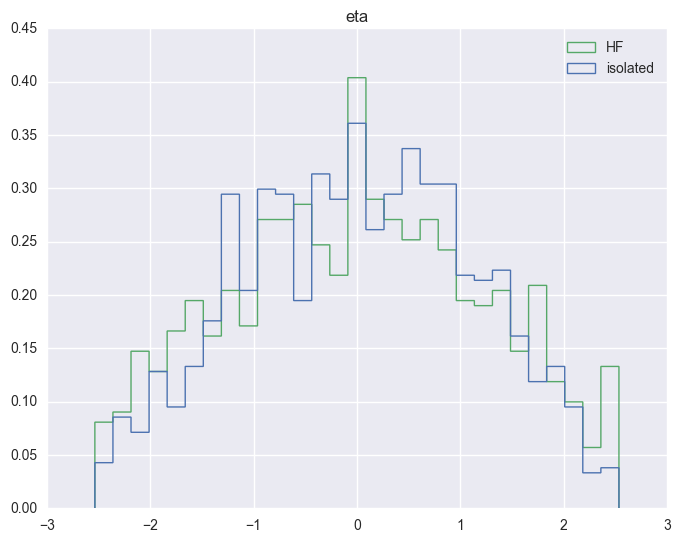
\includegraphics[width=0.45\textwidth]{Images/RNN/lep_eta.png}
    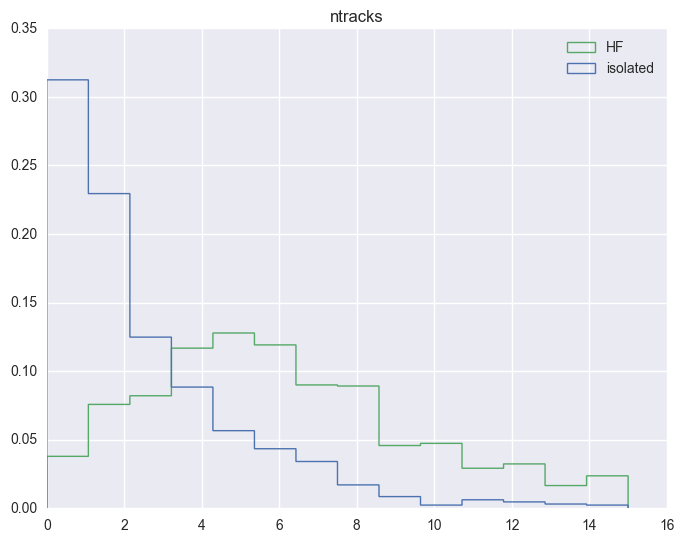
\includegraphics[width=0.45\textwidth]{Images/RNN/lep_ntracks.png}
    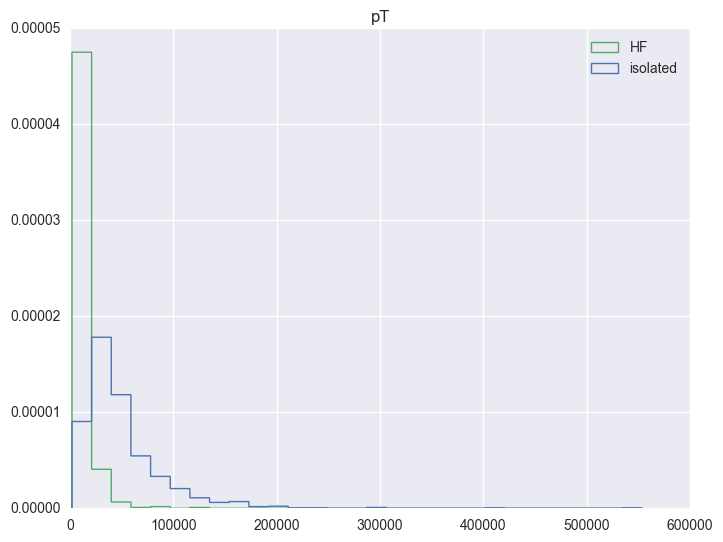
\includegraphics[width=0.45\textwidth]{Images/RNN/lep_pT.png}
    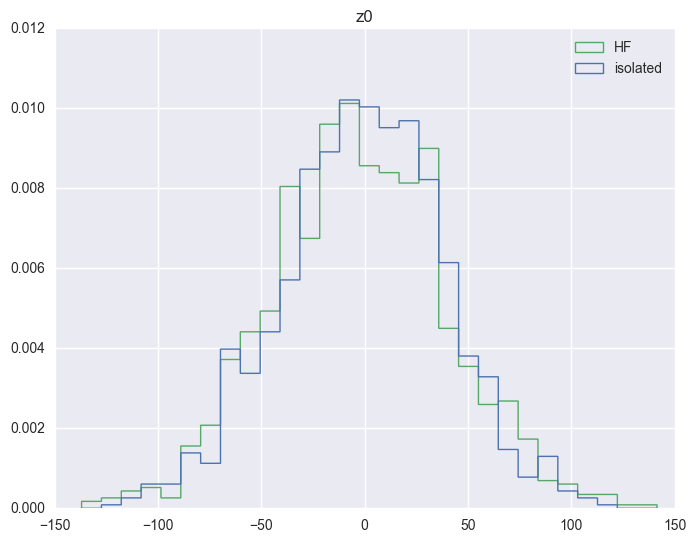
\includegraphics[width=0.45\textwidth]{Images/RNN/lep_z0.png}
    \caption{Comparisons of some features between isolated and heavy-flavor leptons.}
    \label{fig:lep_features}
\end{figure}

\begin{figure}[htbp]
    \centering
    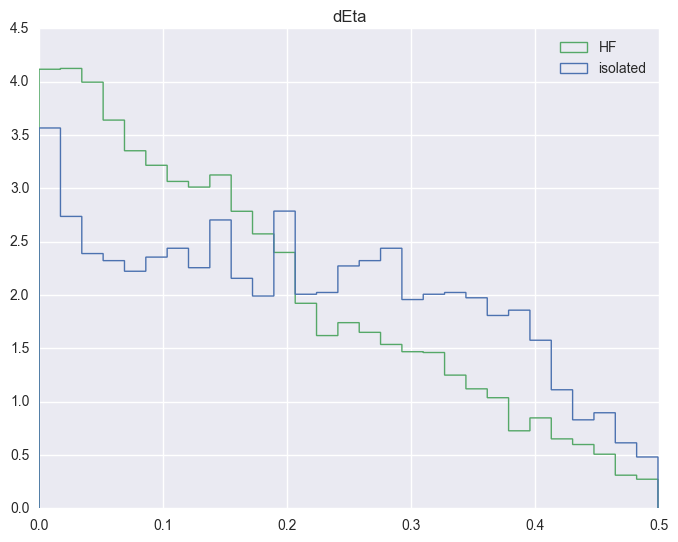
\includegraphics[width=0.45\textwidth]{Images/RNN/track_dEta.png}
    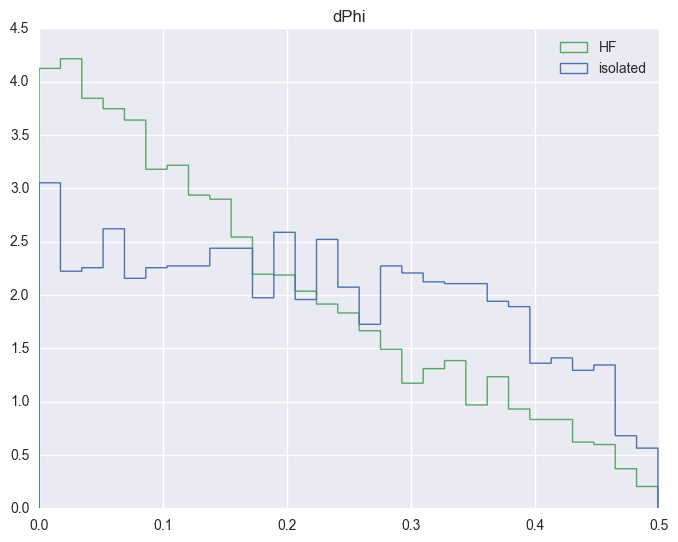
\includegraphics[width=0.45\textwidth]{Images/RNN/track_dPhi.png}
    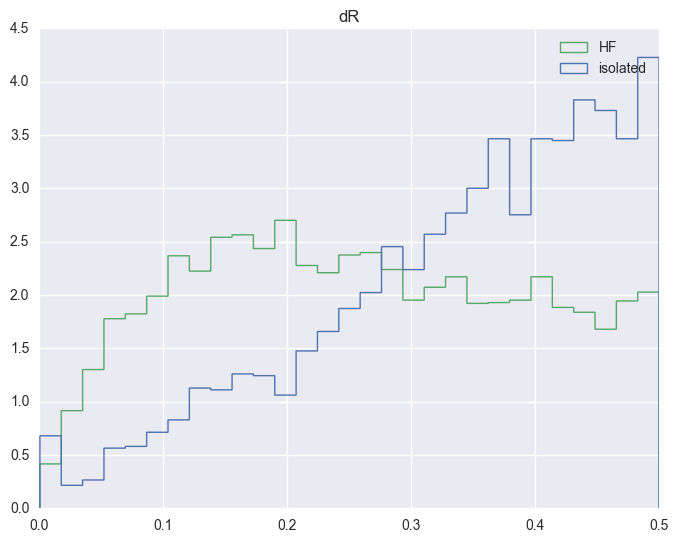
\includegraphics[width=0.45\textwidth]{Images/RNN/track_dR.png}
    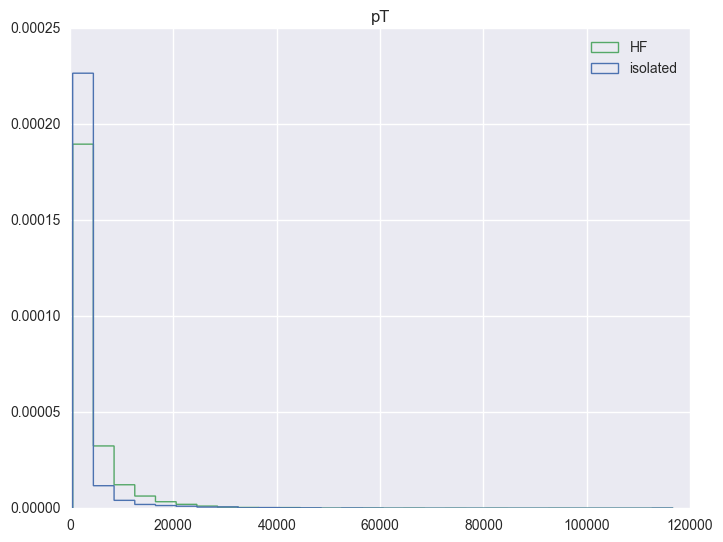
\includegraphics[width=0.45\textwidth]{Images/RNN/track_pT.png}
    \caption{Comparisons of some features between tracks associated with isolated and heavy-flavor leptons.}
    \label{fig:track_features}
\end{figure}

Next, to demonstrate that our object selections are performed correctly, and are appropriate for comparison with existing techniques, we recalculated several cone-based values using our filtered objects. Our recalculated values are compared against the values provided by the cone-based tools in Figure~\ref{fig:cone_compare}.

\begin{figure}[htbp]
    \centering
    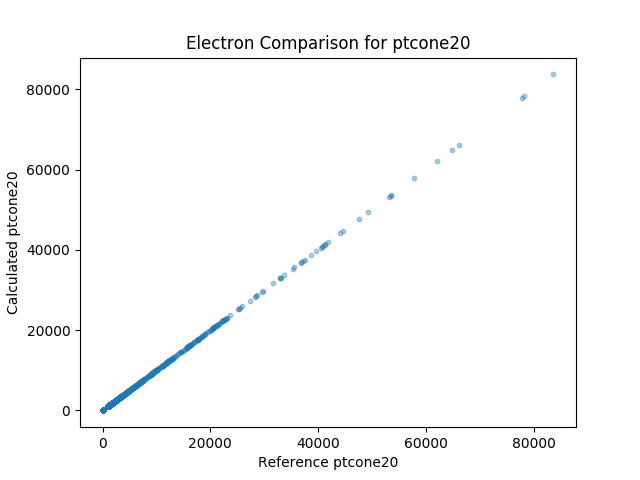
\includegraphics[width=0.45\textwidth]{Images/RNN/electron_ptcone20.png}
    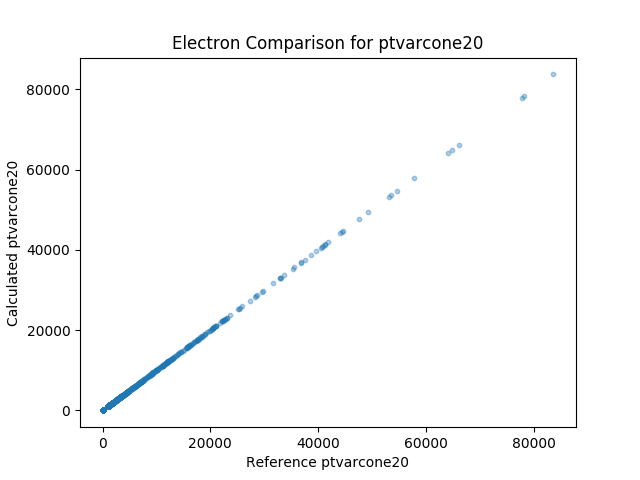
\includegraphics[width=0.45\textwidth]{Images/RNN/electron_ptvarcone20.png}
    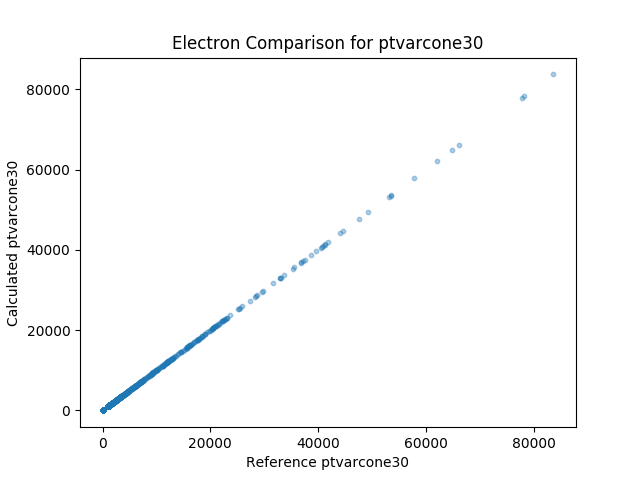
\includegraphics[width=0.45\textwidth]{Images/RNN/electron_ptvarcone30.png}
    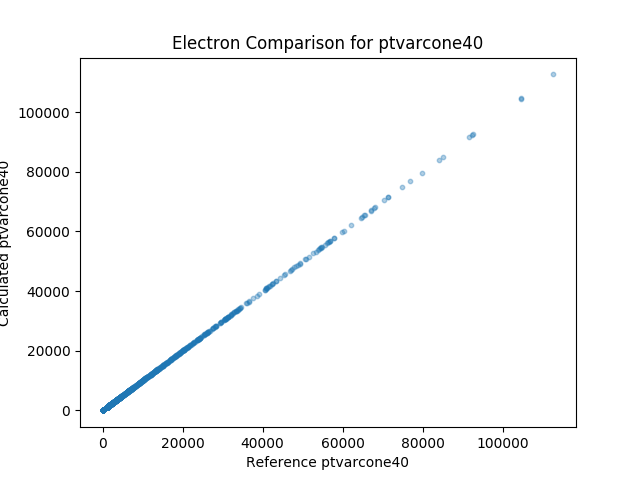
\includegraphics[width=0.45\textwidth]{Images/RNN/electron_ptvarcone40.png}
    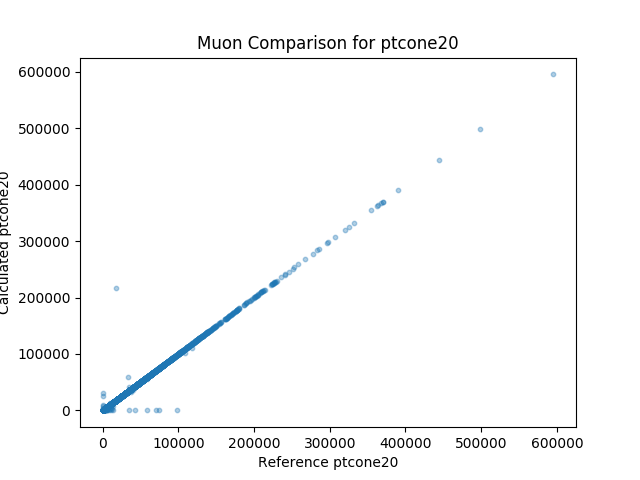
\includegraphics[width=0.45\textwidth]{Images/RNN/muon_ptcone20.png}
    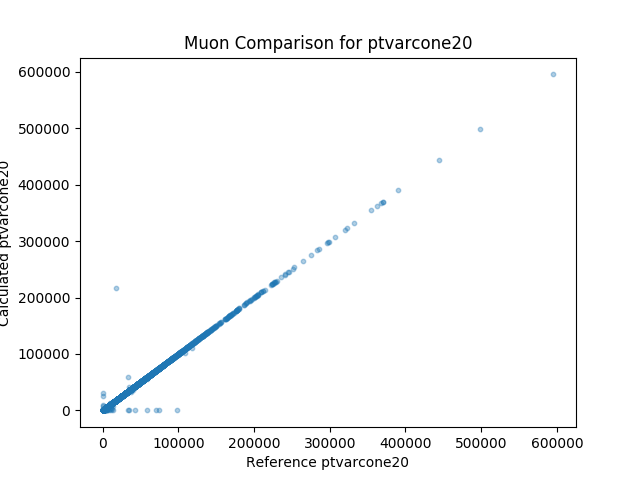
\includegraphics[width=0.45\textwidth]{Images/RNN/muon_ptvarcone20.png}
    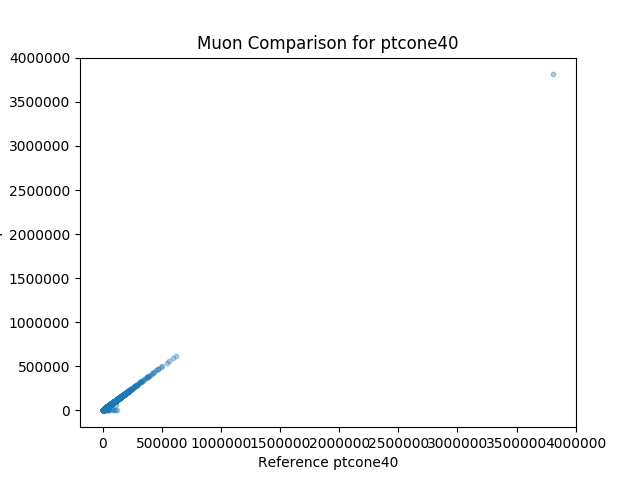
\includegraphics[width=0.45\textwidth]{Images/RNN/muon_ptcone40.png}
    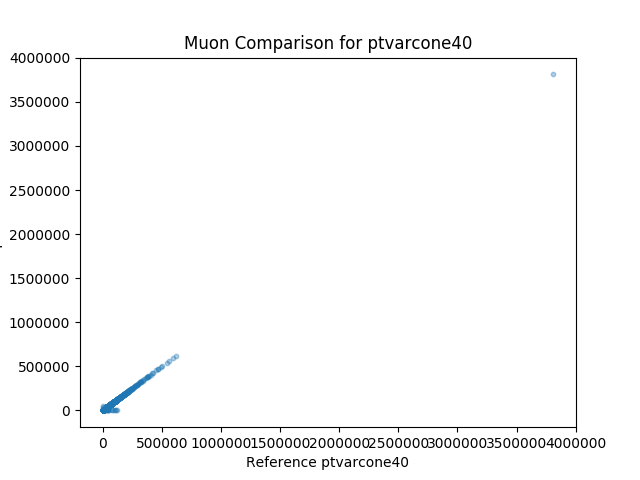
\includegraphics[width=0.45\textwidth]{Images/RNN/muon_ptvarcone40.png}
    \caption{Comparisons of cone-based values, as provided by the official tools, and as recalculated using our objects. We have a mismatch of about $0.1\%$ for muons only. This demonstrates that our object selection is proper for comparison with existing techniques.}
    \label{fig:cone_compare}
\end{figure}

\chapter{Results and Future Work}

We decided to first use a recurrent neural net to approach this problem due to the variable number of tracks associated with each lepton. This naturally led to the question of how to order the tracks. We performed experiments with multiple types of ordering, including in increasing energy, in decreasing energy, in increasing $\Delta R$ from the lepton, and in decreasing $\Delta R$. We found that the ordering didn't really have too much of an effect on the final performance, which is sensible due to the somewhat low number of typical tracks associated with each lepton.

We also looked at using different types of net architectures, including a basic RNN, an LSTM, and a GRU. On top of that we also looked at non-ordered variable-input-size architectures, including deep sets and set transformers. These studies are still ongoing, but the current best results are shown in Figure~\ref{fig:RNN_results}.

\begin{figure}[htbp]
    \centering
    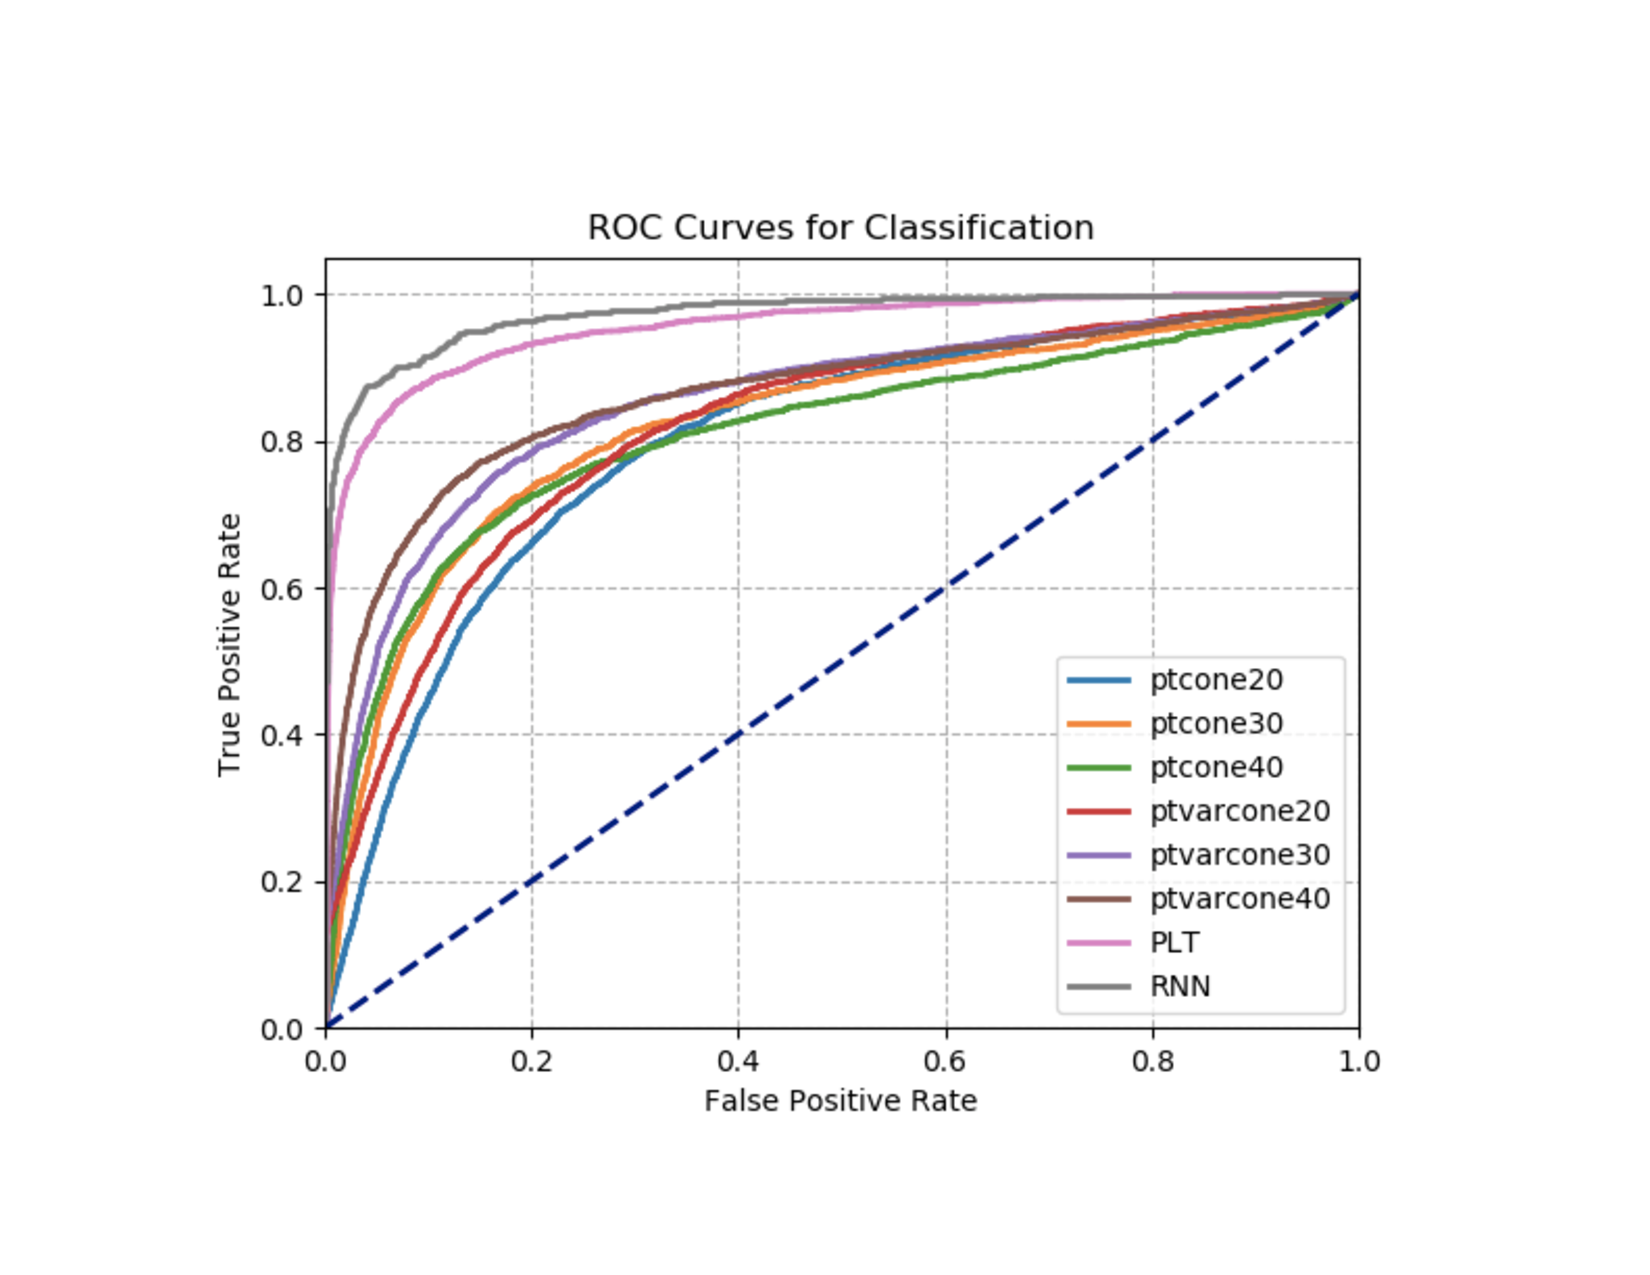
\includegraphics[trim=0 70 0 70, clip,width=\textwidth]{Images/RNN/ROC.pdf}
    \caption{ROC results using our current best architecture, compared against results from cone-based algorithms, and against PLT. These results have been superceded due to recent upgrades to PLT, so the gap in performance is now much smaller.}
    \label{fig:RNN_results}
\end{figure}

These results have been superceded in recent months due to updates to PLT, where the algorithm now also uses an RNN algorithm as one of its BDT inputs. In particular, the algorithm now uses an RNN-based b-tagger, which uses much of the track information we depend on. Thus, the gap in performance is now much smaller than shown in Figure~\ref{fig:RNN_results}. However, we hope to regain a performance gap when we integrate the calorimeter information into the net.

The grad students now in charge of the project are currently looking at methods of combining track and calorimeter information beyond simply having two separate nets connected by a linear final layer. We are also investigating a change in scope of the project, to specifically target soft leptons, which the PLT is weakly sensitive to.